\documentclass[11pt]{article}
\usepackage[margin=0.9in]{geometry}
\usepackage{booktabs,graphicx,float,amsmath,xcolor,enumitem}
\usepackage[hidelinks]{hyperref}
\usepackage{titlesec}
\titleformat{\section}{\large\bfseries}{\thesection.}{0.5em}{}
\titlespacing*{\section}{0pt}{8pt}{3pt}
\setlength{\parindent}{0pt}
\setlength{\parskip}{4pt}
\setlist{nosep,leftmargin=1.2em}
\newcommand{\taurct}{\hat\tau^{\,\mathrm{RCT}}}
\newcommand{\taunaive}{\hat\tau^{\,\mathrm{naive}}}

\begin{document}

{\Large\bfseries Weekly Project Progress Report, Week 7: Do City Chiefs Grant More Discretionary Tax Exemptions?}

\vspace{2pt}
\textbf{Name:} Tsu Ning Tsao \quad \textbf{Student Number:} 1012713137

\section*{One-Paragraph Research Summary}
\textbf{Research question.} When neighbourhood chiefs (Local) instead of state agents (Central) collect the property tax, do more properties get exempted, and are the extra exemptions justified by the owner's legal status or are they discretionary favours? Later weeks ask for which households the effect is larger (e.g.\ co-ethnic owners). \textbf{Data.} Replication data of Bal\'an et al.\ (2022): the 2018 property-tax campaign in Kananga, D.R.\ Congo. Neighbourhoods (\texttt{a7}) were randomly assigned to Central (\texttt{tmt}=1) or Local (\texttt{tmt}=2). The unit is the property: the collectors' registration record merged with an independent monitoring survey of the owner. The full experimental sample is the 5,645 properties in 202 neighbourhoods with exemption status and owner traits recorded. \textbf{Variables.} Outcome $Y$ = \texttt{exempt} (1 if the collector registered the property as tax-exempt); secondary outcomes split exemptions by stated reason and flag \emph{discretionary} exemptions (reason contradicts the owner's traits: ``elderly'' but owner under 55, the legal threshold, or ``widow'' but owner male). Treatment $D$ = \texttt{local}. Covariates: owner age (the selection variable $S$), female, Luluwa (main tribe), works for the state.

\textbf{Track: RCT.} This week uses the \textbf{biased sample} from Week 6 (Recipe B, $\alpha=0$, $\gamma=1$, $S$ = owner age, seed 1465; 1,328 Central, 1,412 Local) unless a row says ``Full''. Code: \texttt{00\_master/00\_master.py} runs \texttt{01\_preanalysis.py}, \texttt{02\_week6\_benchmark.py} (rebuilds the biased sample) and\\ \texttt{02\_analysis/02\_week7\_matching\_ipw.py}; outputs are in \texttt{03\_output/week7/}.

\section{Propensity score matching and IPW (biased sample)}
\textbf{Model.} The propensity score is a logit of $D$ on $S$ and $X$ (owner age, female, Luluwa, state job), fit on the biased sample. I run both estimators from the slides: (i) nearest-neighbour matching on $\hat e(x)$, one twin with replacement (tied twins averaged, which matters because ages heap at round numbers), for the ATE and the ATT; (ii) IPW, $\hat\tau_{IPW}=\frac1N\sum_{D=1}Y_i/\hat e_i-\frac1N\sum_{D=0}Y_j/(1-\hat e_j)$, plus the normalised (Hajek) version. DoWhy's \texttt{propensity\_score\_matching} and \texttt{propensity\_score\_weighting} are a cross-check; they fit the score on the DAG 2 back-door set, owner age only.

\section{Positivity check (biased sample)}
\begin{figure}[H]\centering
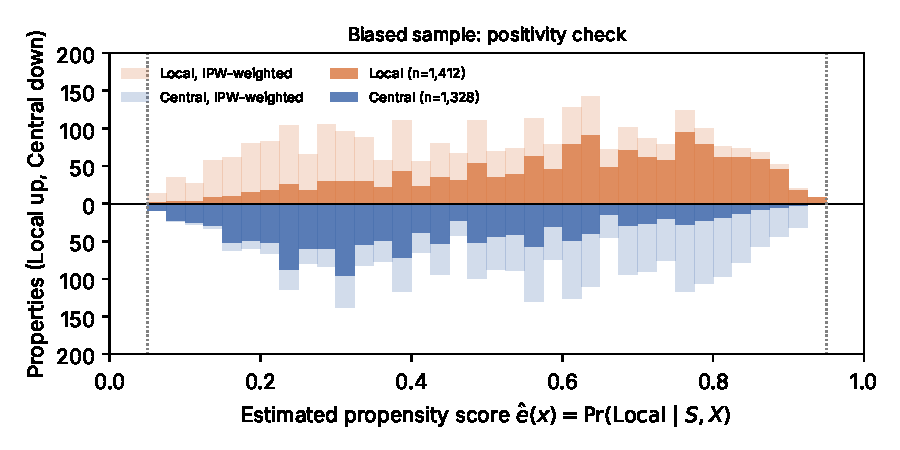
\includegraphics[width=0.72\linewidth]{figure1_positivity.pdf}
\caption{Estimated propensity score, biased sample. Dark bars: Local (up) and Central (down). Light bars: the same units after IPW weighting. Dotted lines at 0.05 and 0.95.}
\end{figure}
\textbf{Positivity holds.} Local scores run from 0.07 to 0.95 and Central scores from 0.06 to 0.91, so the two groups cover the same range; no unit is below 0.05 or above 0.95, and 2.3\% are outside $[0.10, 0.90]$. As expected, Local mass sits at high scores (older owners) and Central at low scores, but both groups appear in every bin except the last one (0.925--0.95), which holds a handful of Local units. The largest IPW weight is 14, the top 1\% of weights carry 4.3\% of the total, and each weighted group sums to about $N$ (2,761 and 2,731 vs 2,740). The selection with $\gamma=1$ is strong enough to bias the naive estimate but not so strong that it breaks overlap, so I keep $\gamma=1$.

\begin{table}[H]\centering\small
\caption{Covariate balance in the biased sample before and after adjustment (standardised mean difference, SMD = difference in means / pooled SD).}
\begin{tabular}{lccccccc}
\toprule
 & Full & \multicolumn{3}{c}{Biased, unweighted} & \multicolumn{2}{c}{After IPW} & After matching\\
\cmidrule(lr){2-2}\cmidrule(lr){3-5}\cmidrule(lr){6-7}\cmidrule(lr){8-8}
Covariate & SMD & Central & Local & SMD & Central/Local & SMD & SMD\\
\midrule
Owner age (S) & -0.022 & 49.8 & 62.8 & 0.967 & 56.4/56.2 & -0.017 & 0.001\\
Owner 55 or older & -0.002 & 0.355 & 0.734 & 0.825 & 0.547/0.546 & -0.001 & 0.004\\
Owner female & -0.063 & 0.228 & 0.289 & 0.139 & 0.264/0.257 & -0.015 & -0.012\\
Owner Luluwa & 0.084 & 0.754 & 0.808 & 0.132 & 0.781/0.781 & -0.000 & -0.009\\
Owner works for state & -0.037 & 0.237 & 0.232 & -0.012 & 0.233/0.231 & -0.004 & -0.031\\
\bottomrule
\end{tabular}

\par\smallskip\footnotesize ``Full'': full experimental sample, unweighted. IPW: Horvitz--Thompson weights $1/\hat e$, $1/(1-\hat e)$. Matching: each unit weighted by $1+K_i$, where $K_i$ is the number of times it is used as a twin.
\end{table}
Selection opened an SMD of 0.97 in owner age (49.8 vs 62.8 years). After weighting or matching every SMD is below 0.04 and owner age is 56.4 vs 56.2: both methods rebuild a sample that looks like the experiment (full-sample SMDs are all below 0.09).

\section{Comparison to the benchmark}
\begin{table}[H]\centering\small
\caption{Effect of Local on \texttt{exempt}. Rows 1--2: full experimental sample; other rows: biased sample.}
\begin{tabular}{lllccc}
\toprule
Sample & Estimator & Target & $\hat\tau$ & SE & 95\% CI\\
\midrule
Full & Benchmark: regression Y on D + S + X ($\hat\tau^{RCT}$) & ATE & 0.031 & 0.026$^c$ & \\
Full & IPW (score on S + X) & ATE & 0.031 &  & \\
\addlinespace
Biased & Difference in means & -- & 0.219 &  & \\
Biased & Naive: regression Y on D + X, no S ($\hat\tau^{naive}$) & -- & 0.200 & 0.032$^c$ & \\
\addlinespace
Biased & PS matching, 1-NN with replacement & ATE & 0.048 & 0.019$^a$ & \\
Biased & PS matching, 1-NN with replacement & ATT & 0.057 & 0.026$^a$ & \\
Biased & IPW, Horvitz--Thompson (divide by $N$) & ATE & 0.033 & 0.031$^b$ & [-0.031, 0.089]\\
Biased & IPW, normalised weights (Hajek) & ATE & 0.030 & 0.028$^b$ & [-0.029, 0.084]\\
\addlinespace
Biased & DoWhy PS matching (score on S only) & ATE & -0.011 &  & \\
Biased & DoWhy IPW, ips\_weight (score on S only) & ATE & 0.024 &  & \\
Biased & Week 6: regression Y on D + S + X & -- & 0.041 & 0.029$^c$ & \\
\bottomrule
\end{tabular}

\par\smallskip\footnotesize $^c$ SE clustered by neighbourhood. $^a$ Abadie--Imbens (2006) SE (score treated as known, not clustered); the bootstrap is not valid for nearest-neighbour matching (Abadie and Imbens 2008). $^b$ Bootstrap SE and 95\% percentile CI: 500 draws resampling neighbourhoods, score re-estimated in each draw, seed 1465.
\end{table}
Against $\taurct=0.031$ and $\taunaive=0.200$: \textbf{IPW gives 0.033 (Hajek 0.030) and removes essentially all of the 17-point selection bias; PS matching gives 0.048 (ATE) and removes about 90\%.} Matching sits a little higher because a twin is only close in $\hat e$, not identical (Abadie--Imbens bias), and the ATT (0.057) averages over Local owners, who are older in this sample. The DoWhy matching estimate ($-0.011$) moves more because it keeps one arbitrary twin among many tied ages; DoWhy IPW (0.024) agrees with mine. As a sanity check, IPW on the full sample gives 0.031, the same as $\taurct$: with random $D$ there is nothing to correct.

\textbf{Recipe B check.} Recipe B implies $\operatorname{logit}\Pr(D=1\mid S,\text{kept}) = \log\frac{p}{1-p} + \gamma S$, because $\Lambda(\gamma S)/\Lambda(-\gamma S)=e^{\gamma S}$ ($p$ = Local share in the full sample).
\begin{table}[H]\centering\small
\caption{Logit of $D$ on standardised $S$ (full-sample mean and SD, as in the recipe), biased sample, SE clustered by neighbourhood.}
\begin{tabular}{lcccc}
\toprule
Logit model (biased sample) & $\hat\gamma$ (coef.\ on std.\ $S$) & SE & Constant & $N$\\
\midrule
D on S\_std & 1.042 & 0.066 & 0.052 & 2,740\\
D on S\_std + X & 1.052 & 0.064 & -0.122 & 2,740\\
Recipe B (true value) & 1.000 & & 0.044 & \\
\bottomrule
\end{tabular}

\end{table}
$\hat\gamma = 1.04$ (95\% CI $[0.91, 1.17]$) against the true $\gamma=1$: same sign, same size, and the constant (0.05) matches $\log(p/(1-p))=0.04$. Adding $X$ leaves it at 1.05 and none of $X$ predicts $D$ (all $p\ge0.19$), consistent with DAG 2 where only $S$ points into $D$.

\section{Bootstrap (optional step, done)}
\begin{figure}[H]\centering
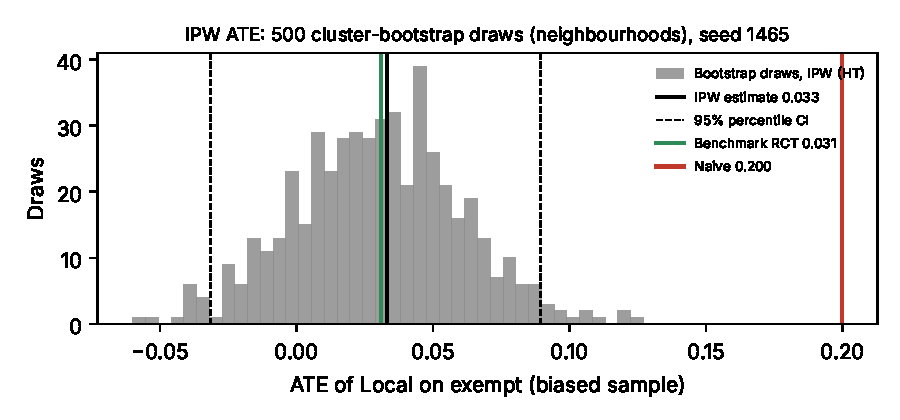
\includegraphics[width=0.72\linewidth]{figure2_bootstrap_ipw.pdf}
\caption{Bootstrap distribution of the IPW ATE, biased sample. 500 draws resampling neighbourhoods (the unit of randomisation), propensity score re-estimated in every draw, seed 1465.}
\end{figure}
The bootstrap SE is 0.031 and the 95\% CI is $[-0.031, 0.089]$: it contains $\taurct=0.031$ and is far from $\taunaive=0.200$. Like the benchmark, the corrected effect on exemptions is small and not significant.

\section{What I learned}
Once owner age is in the score, both matching and IPW undo the selection I built: balance is restored (all SMD $<0.04$) and the estimate returns from 0.200 to 0.03--0.05. It works here because I know the selection rule and $S$ is observed; in real observational data, the chief's personal ties to the owner would be an unobserved confounder that neither method can fix. Next week the propensity score returns in the meta-learners, which I will use to ask whether the Local effect on exemptions is larger for co-ethnic owners.

\end{document}
